\documentclass[10pt,a4paper]{article}
\usepackage[english,greek]{babel}
\usepackage[utf8x]{inputenc}
\usepackage{graphicx}

\begin{document}

\title{Αρχιτεκτονική Υπολογιστών \\ 
	\begin{small}
	Τμήμα Μηχανικών Πληροφορικής και Τηλεπικοινωνιών \\ Εργασία Τρίτου Εξαμήνου
	\end{small}}
\maketitle

\begin{small}
	\subsubsection*{Μέλη της ομάδας}
		\begin{enumerate}
		\item Ανέστης Δαλγκίτσης, 586, 3ο εξάμηνο
		\item Γεώργιος Θεόδωρος Καλαμπόκης, 594, 3ο εξάμηνο
		\item Χρήστος Παλαμιώτης, 648, 3ο εξάμηνο
		\item Χρήστος Τόλης, 632, 3ο εξάμηνο
	\end{enumerate}
\end{small}

\section*{Εισαγωγή}
\begin{itemize}
\item Το πρόγραμμα της ομάδας μας ελέγχει την εγκυρότητα πιστωτικών καρτών τύπου:
\latintext 
\begin{itemize}
\item Mastercard
\item VISA
\item Amex
\item Diners Club
\item Discover
\end{itemize}
\greektext

\item Επίσης ως πρόσθετη λειτουργία έχει την δυνατότητα να δημιουργεί κάρτες των ίδιων τύπων ανάλογα με την προτίμηση του χρήστη.

\item Η είσοδος για τον έλεγχο των καρτών γίνεται με ένα αρχείο \latintext txt \greektext που βρίσκεται στον ίδιο φάκελο με το εκτελέσιμο αρχείο
\end{itemize}

\subsubsection*{Δυνατότητες}
\begin{itemize}
\item Ο χρήστης μπορεί να εισάγει όσες κάρτες επιθυμεί προς έλεγχο στο αρχείο \latintext txt\greektext , καθώς δεν υπάρχει περιορισμός.
\item Υπάρχει έλεγχος για μη έγκυρους χαρακτήρες (όπως γράμματα και σύμβολα). Στην περίπτωση ύπαρξής τους, ο χρήστης ενημερώνεται με το κατάλληλο μήνυμα.
\end{itemize}

\subsubsection*{Απαιτήσεις για ορθή λειτουργία}
\begin{itemize}
\item Το αρχείο \latintext txt \greektext πρέπει να βρίσκεται στον ίδιο φάκελο με το εκτελέσιμο αρχείο (ή στον φάκελο του debugger αν εκτελεστεί προσομοίωση με το emu8086).
\item Το αρχείο \latintext txt \greektext θα πρέπει να είναι κωδικοποίησης \latintext ANSI \greektext ή \latintext UTF-8 \greektext.
\item Όλες οι κάρτες πρέπει να αναγράφονται \textbf{ΧΩΡΙΣ} κενά (πχ: 30569309025904) και να αναγράφονται \textbf{μία ανά γραμμή}.
\item Ο μέγιστος αριθμός ψηφίων ανά κάρτα είναι 255 αριθμοί.
\end{itemize}

\section*{Οδηγός χρήσης}

\subsubsection*{Πριν την εκτέλεση}
\begin{enumerate}
\item Δημιουργούμε ένα αρχείο με όνομα \latintext cards.txt \greektext και το αποθηκεύουμε στον ίδιο φάκελο με το εκτελέσιμο αρχείο, σύμφωνα με τους περιορισμούς του προγράμματος.
\item Αναγράφουμε τους αριθμούς των πιστωτικών καρτών προς έλεγχο εγκυρότητας σύμφωνα με τους περιορισμούς του προγράμματος.
\end{enumerate}

\begin{center}
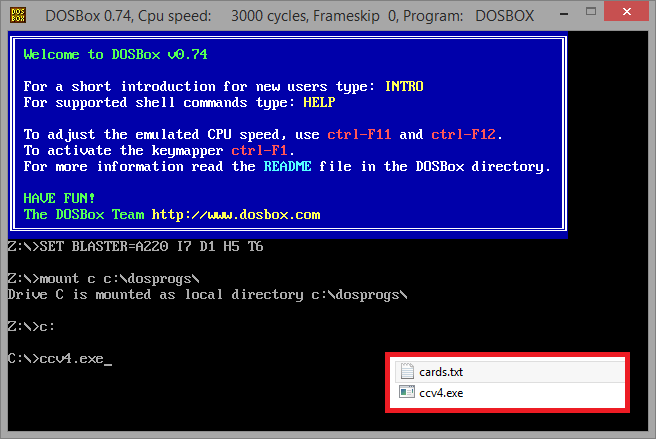
\includegraphics[scale=0.7]{cdosboxloadext.PNG}
\end{center}

\pagebreak

\subsubsection*{Εκτέλεση}
\begin{enumerate}
\item Κατά την εκκίνηση του προγράμματος τυπώνεται στην οθόνη ένα σχέδιο κατασκευασμένο από χαρακτήρες \latintext ASCII \greektext που φανερώνει το όνομα του προγράμματός μας \latintext (CCV\_4, \greektext δηλαδή \latintext Credit Card Validator version 4) \greektext καθώς και τα ονόματα των προγραμματιστών της ομαδας μας.
\item Για συνέχεια πατάμε τον χαρακτήρα \latintext ENTER (RETURN)\greektext.
\end{enumerate}

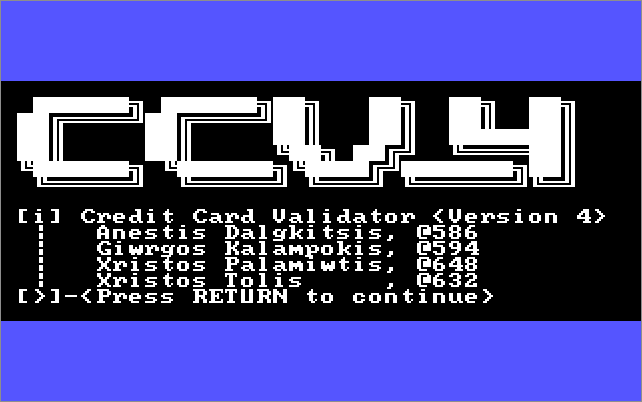
\includegraphics[scale=0.7]{csplash.PNG}

\subsubsection*{Κεντρικό μενού επιλογών}
\begin{enumerate}
\item Στη συνέχεια εμφανίζεται ένα γραφικό περιβάλλον επιλογών.
\item Εδώ ο χρήστης καλείται να επιλέξει να επιλέξει ποια λειτουργία θέλει να εκτελέσει
	\begin{enumerate}
	\item Πατώντας τον αριθμό 1, το πρόγραμμα μεταβαίνει στην οθόνη ελέγχου εγκυρότητας των πιστωτικών καρτών που αναγράφονται στο αρχείο \latintext cards.txt\greektext.
	\item Πατώντας τον αριθμό 2, το πρόγραμμα μεταβαίνει στην οθόνη δημιουργίας πιστωτικών καρτών.
	\item Με τον αριθμό 3 τερματίζεται η εκτέλεση του προγράμματος
	\item Ενώ με τον αριθμό 4 τυπώνεται η αρχική οθόνη.
	\end{enumerate}
\end{enumerate}

\begin{center}
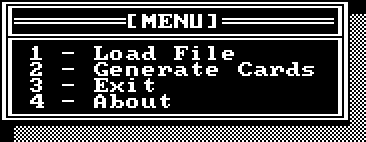
\includegraphics[scale=0.8]{cmenucrop.PNG}
\end{center}

\subsubsection*{Οθόνη ελέγχου εγκυρότητας πιστωτικών καρτών}
\begin{enumerate}
\item Σε αυτή τη λειτουργία εμφανίζονται τα αποτελέσματα του ελέγχου εγκυρότητας των πιστωτικών καρτών που αναγράφονται στο αρχείο \latintext cards.txt\greektext.
	\begin{enumerate}
	\item Τα αποτελέσματα εμφανίζονται με την σειρά που έχουν οι κάρτες.
	\item Στην περίπτωση έγκυρης κάρτας, αναγράφονται ο αριθμός της κάρτας καθώς και ο τύπος της.
	\item Σε περίπτωση μη έγκυρης κάρτας, αναγράφεται ο αριθμός της καθώς και το αντίστοιχο μήνυμα μη-εγκυρότητας.
	\item Σε περίπτωση μη αποδεκτών χαρακτήρων (δηλαδή συμβόλων, γραμμάτων και κενών χαρακτήρων), εμφανίζεται μόνο το μήνυμα μη έγκυρης εισόδου.
	\item Η φόρτωση και ο έλεγχος νέας κάρτας γίνεται πατώντας το πλήκτρο \latintext ENTER (RETURN)\greektext.
	\item Η διαδικασία επαναλαμβάνεται μέχρι και τον έλεγχο της τελευταίας κάρτας.
	\item Αφού τελειώσει η διαδικασία, εμφανίζεται και πάλι το κεντρικό μενού επιλογών.
	\end{enumerate}
\end{enumerate}

\begin{center}
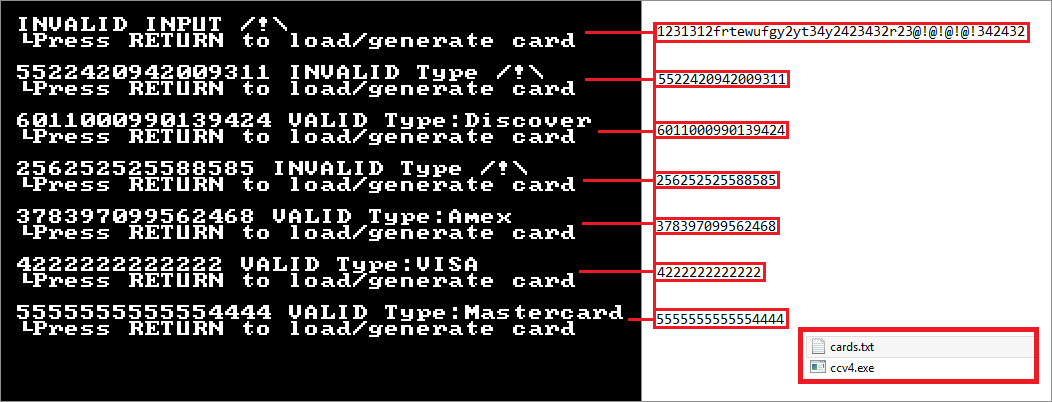
\includegraphics[scale=0.5]{cloaddesc.PNG}
\end{center}

\pagebreak

\subsubsection*{Οθόνη δημιουργίας πιστωτικών καρτών}
\begin{itemize}
\item Σε αυτή τη λειτουργία ο χρήστης καλείται να επιλέξει τον τύπο και της/των πιστωτικής/πιστωτικών κάρτας/καρτών καθώς και τον αριθμό των καρτών που θέλει να δημιουργήσει.
	\begin{enumerate}
	\item Αρχικά ο χρήστης επιλέγει τον τύπο των καρτών με τα πλήκτρα 0 εώς 4, σύμφωνα με τις οδηγίες που δείχνει η οθόνη.
	\item Στην συνέχεια επιλέγει τον αριθμό των καρτών που θέλει να δημιουργήσει. \textbf{Προσοχή!} Ο αριθμός αυτός είναι τριψήφιος. Για παράδειγμα εάν ο χρήστης θέλει να δημιουργήσει 9 κάρτες θα πρέπει να γράψει 009.	
	\end{enumerate}
	
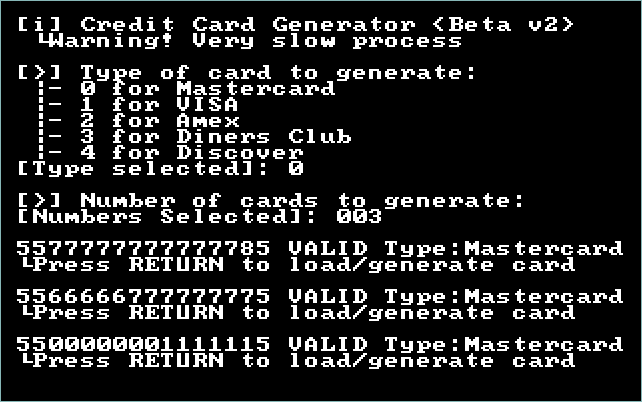
\includegraphics[scale=0.75]{cload.PNG}

\item \textbf{Προσοχή! Η δημιουργία έγκυρων πιστωτικών καρτών είναι πολύ χρονοβόρα και μπορεί να διαρκέσει από μερικά δευτερόλεπτα μέχρι μερικά λεπτά.} 
\item Το αίτημα για δημιουργία και εμφάνιση νέας κάρτας γίνεται πατώντας το πλήκτρο \latintext ENTER (RETURN)\greektext.
\item \textit{Προτείνεται το αίτημα για νέα κάρτα να γίνεται μετά από λίγα δευτερόλεπτα από την εμφάνιση της προηγούμενης κάρτας}
\item Η διαδικασία επαναλαμβάνεται μέχρι και την δημιουργία της τελευταίας κάρτας.
\item Αφού τελειώσει η διαδικασία, εμφανίζεται και πάλι το κεντρικό μενού επιλογών.
\end{itemize}

\section*{Περιγραφή Αλγορίθμων \& Σημαντικά κομμάτια κώδικα}
Το πρόγραμμα αυτό δημιουργήθηκε με βάση κάποιους κανόνες σχετικά με τον διαχωρισμό των λειτουργιών σε διάφορες συναρτήσεις και την επαναχρησιμοποίηση κώδικα

\subsubsection*{Η συνάρτηση \latintext readfile}
\begin{itemize}
\item Ανοίγει μια ροή \latintext (stream) \greektext μόνο για την ανάγνωση \latintext (read-only) \greektext του αρχείου \latintext cards.txt \greektext ανά \latintext byte\greektext, με την βοήθεια της διακοπής \latintext INT 21h \greektext του λειτουργικού συστήματος \latintext DOS\greektext.
\item Λειτουργεί με έναν κεντρικό βρόγχο επανάληψης \latintext readloop \greektext ο οποίος εκτελείται μέχρι και το τελευταίο \latintext byte \greektext του αρχείου.
	\begin{itemize}
	\item Μέσα σε αυτόν τον βρόγχο εκτελούνται έλεγχοι εγκυρότητας εισόδου, οι μετατροπές των έγκυρων χαρακτήρων \latintext ASCII \greektext σε αριθμούς καθώς και η αποθήκευση αυτών στον πίνακα \latintext cardnum[255]\greektext.
	\end{itemize}
\item Μόλις ολοκληρωθεί η ανάγνωση μιας έγκυρης γραμμής - κάρτας, προχωράμε στον έλεγχο του τύπου της κάρτας με την κλήση της συνάρτησης \latintext credit\_card\_type\_finder \greektext και έπειτα στον έλεγχο της εγκυρότητας της κάρτας με την κλήση της συνάρτησης \latintext LUHNv \greektext (αλγόριθμος \latintext LUHN (mod 10)\greektext). Τέλος εκτελείται η τύπωση των αποτελεσμάτων από την συνάρτηση \latintext printcards\greektext.
\end{itemize}

\subsubsection*{Η συνάρτηση \latintext card\_generator\_menu}
\begin{itemize}
\item Η \latintext card\_generator\_menu \greektext δέχεται από τον χρήστη τον τύπο  καθώς και τον αριθμό των καρτών που θέλει να δημιουργήσει.
\item Αφού ο χρήστης εισάγει τις προτιμήσεις του εκτελείται ένας βρόγχος επανάληψης ο οποίος για κάθε κάρτα καλεί τις κατάλληλες συναρτήσεις για την δημιουργία και την εμφάνιση των καρτών.
	\begin{itemize}
	\item Μέσα σε αυτόν καλείται η συνάρτηση \latintext card\_generator\greektext η οποία επιλέγει το κατάλληλο πρόθεμα και μήκος ανάλογα με τον τύπο της κάρτας.
	\item Οι υπόλοιποι αριθμοί της κάρτας επιλέγονται τυχαία απο την συνάρτηση \latintext Pseudonoise\_Number\_Generator\greektext. Στην πραγματικότητα οι τιμές αυτές υπολογίζονται με βάση την ώρα και την ημερομηνία του συστήματος.
	\item Αφού έχει δημιουργηθεί μια τυχαία κάρτα καλείται ο αλγόριθμος του \latintext LUHN \greektext για την επιβεβαίωση της έγκυρης τιμής. Αν ο αριθμός της τυχαίας κάρτας δεν είναι έγκυρος σύμφωνα με τον \latintext LUHN \greektext η διαδικασία επαναλαμβάνεται.
	\item Μόλις ο \latintext LUHN \greektext εγκρίνει την τυχαία κάρτα καλείται η συνάρτηση \latintext printCards \greektext η οποία τυπώνει τον αριθμό και τον τύπο της.
	\end{itemize}
\end{itemize}

\subsubsection*{Συναρτήσεις διαχείρισης γραφικών \latintext VGA }
\begin{itemize}
\item Με την εκκίνηση του προγράμματος εκτελείται η συνάρτηση \latintext setgraphics \greektext που μεταβάλει την ανάλυση της οθόνης για την σωστή τύπωση των γραφικών. Με την λήξη του προγράμματος κάθε γραφικό στοιχείο και χαρακτήρας \latintext ASCII \greektext απομακρύνεται με την συνάρτηση \latintext optimiseScreen \greektext και στην συνέχεια το σύστημα ανακτά την προεπιλεγμένη ανάλυση.
\item Η συνάρτηση \latintext splashscreen \greektext δημιουργεί 2 γαλάζια πλαίσια στο πάνω και στο κάτω μέρος της οθόνης, γράφοντας στην μνήμη \latintext VGA \greektext τα αντίστοιχα \latintext pixels \greektext τους. Στη συνέχεια τυπώνεται το όνομα του προγράμματος με χαρακτήρες \latintext ASCII \greektext καθώς και τα στοιχεία των μελών της ομάδας μας.
\item Η συνάρτηση \latintext menu \greektext πέραν από τις λειτουργίες επιλογής και ελέγχου, είναι εξ ολοκλήρου κατασκευασμένη με χαρακτήρες \latintext ASCII \greektext.
\end{itemize}

\section*{Δείκτες απόδοσης}

\subsubsection*{Σημαντικά μεγέθη κώδικα}
\begin{itemize}
\item Μέγεθος αρχείου πηγαίου κώδικα: 25 \latintext KB \greektext
\item Μέγεθος αρχείου εκτελέσιμου αρχείου: 4 \latintext KB \greektext
\item Μεγέθη κώδικα
\latintext
	\begin{itemize}
	\item Code Segment: 1566 bytes
	\item Data Segment: 1434 bytes
	\item Stack Segment: 256 bytes
	\end{itemize}
\greektext
\end{itemize}

\subsubsection*{Μη αποδοτικά κομμάτια κώδικα}
\begin{enumerate}
\item Η συνάρτηση \latintext cards\_generator \greektext
	\begin{itemize}
	\item Έχει κατασκευαστεί με τέτοιο τρόπο ώστε να καλείται διαρκώς η συνάρτηση που εκτελεί τον αλγόριθμο \latintext LUHN\greektext, μέχρι να βρεθεί μια τυχαία κάρτα που τον ικανοποιεί. Αυτό έχει ως αποτέλεσμα για την παραγωγή μιας κάρτας να χρειαστεί να κληθεί μέχρι και μερικές εκατοντάδες φορές καθιστώντας την όλη διαδικασία υπερβολικά αργή και χρονοβόρα.
	\item Το πρόβλημα της καθυστέρησης επιτείνεται όταν η ώρα δεν επιτρέπει την παραγωγή των επιθυμητών “τυχαίων” αριθμών. Αυτό συμβαίνει διότι οι τυχαίοι αριθμοί παράγονται με βάση τα δευτερόλεπτα της ώρας \latintext (wall clock time) \greektext καθώς δεν υπάρχει κάποια εντολή στον 8086 για την επιστροφή τυχαίων αριθμών. Στη συγκεκριμένη περίπτωση η διαδικασία καθυστερεί περισσότερο από ένα λεπτό και αφήνει τον χρήστη να πιστεύει πως η εφαρμογή δεν αποκρίνεται, κάτι που δεν ισχύει. Περισσότερες πληροφορίες σχετικά με το πρόβλημα αυτό θα βρείτε στην τελευταία σελίδα αυτού του εγγράφου.
	\end{itemize}
\item Η συνάρτηση \latintext Pseudonoise\_Number\_Generator \greektext
	\begin{itemize}
	\item Η συνάρτηση αυτή αποτελεί το λιγότερο αποδοτικό κομμάτι του κώδικα καθώς καλείται το λιγότερο 13 φορές για να δημιουργήσει μια κάρτα. Τις περισσότερες φορές ο αλγόριθμος \latintext LUHN \greektext απορρίπτει την κάρτα που μόλις δημιουργήθηκε και έτσι επαναλαμβάνεται η όλη διαδικασία. 
	\item Μέσα στην συνάρτηση αυτή υπάρχει ο βρόγχος \latintext pseudoLoop \greektext ο οποίος επαναλαμβάνεται κάθε φορά που ο τυχαίος αριθμός είναι μεγαλύτερος του 9. Στατιστικά επαναλαμβάνεται 2 από τις 6 φορές.
	\item Τέλος, το πέρασμα της τυχαίας τιμής γίνεται μέσω του τμήματος δεδομένων, μειώνει ελάχιστα την ταχύτητα εκτέλεσης.
	\end{itemize}
\end{enumerate}

\subsubsection*{Αξιοσημείωτες τεχνικές προγραμματισμού}
\begin{itemize}
\item Χρησιμοποιήθηκαν καταχωρητές μέσα σε βρόγχους που εκτελούνται πάρα πολλές φορές.
\item Οι περισσότερες μετακινήσεις δεδομένων μεταξύ μνήμης και καταχωρητών γίνονται πριν την είσοδο στους βρόγχους
\item Συγκεκριμένοι πολλαπλασιασμοί και διαιρέσεις γίνονται με την λειτουργία \latintext shift \greektext για γρηγορότερα αποτελέσματα
\item Η αρχικοποίηση των 16  \latintext bit \greektext καταχωρητών αντικαταστάθηκε με την εντολή \latintext XOR \greektext για ταχύτερη εκτέλεση και μικρότερη επιβάρυνση σε \latintext bytes \greektext.
\end{itemize}

\subsubsection*{Σχετικά με την διασωλήνωση}
\begin{itemize}
\item Το πρόγραμμα αυτό έχει σχεδιαστεί για να εκτελείται στον επεξεργαστή 8086 της \latintext Intel \greektext ο οποίος δεν υποστηρίζει διασωλήνωση. 
\item Ενδεικτικά αναφέρονται κάποια παραδείγματα κινδύνων διασωλήνωσης
	\latintext
	\begin{enumerate}
	\item RAW (Read After Write)\\ADD CL,CH\\MOV sum,CL
	\item WAR (Write After Read)\\MOV BH,cardnum[DI]\\MOV cardnum[SI],BH 
	\item WAW (Write After Write)\\MOV AL,cardnum[SI]\\ADD AL,AL
	\end{enumerate}
	\greektext
\end{itemize}

\section*{Προβλήματα κατά την υλοποίηση και επίλυση αυτών}

\subsubsection*{Πρόβλημα με τον έλεγχο εισόδου και η λύση του}

	Ένα σημαντικό πρόβλημα εμφανίστηκε κατά την δοκιμαστική εκτέλεση του προγράμματος, καθώς αυτό δεν διάβαζε την κάρτα που βρίσκονταν γραμμένη στην τελευταία γραμμή του αρχείου \latintext cards.txt\greektext. Το πρόβλημα αντιμετωπίστηκε ελέγχοντας αν το τελευταίο byte που διαβάστηκε είναι ο χαρακτήρας newline ή \latintext 0xA\greektext. Σε αυτή την περίπτωση διαβάζεται ακόμη μια γραμμή, δηλαδή η τελευταία. Υπάρχει ξεχωριστός έλεγχος ώστε να μην διαβαστούν και άλλα \latintext bytes \greektext που δεν ανήκουν στο αρχείο.

\subsubsection*{Το πρόβλημα με την “γέννηση” πραγματικά τυχαίων αριθμών}

	Ένα πολύ σημαντικό πρόβλημα που παρουσιάστηκε είναι η παραγωγή πραγματικά τυχαίων αριθμών. Μετά από αρκετή ώρα αναζήτησης στο \latintext internet \greektext όπως και στις διαφάνειες του μαθήματος, διαπιστώσαμε πως όσοι αλγόριθμοι ψευδοτυχαίων αριθμών δοκιμάσαμε μας έδιναν συνεχώς τον ίδιο αριθμό και συνεπώς, τις ίδιες κάρτες. Αυτό συμβαίνει γιατί όλοι αυτοί οι αλγόριθμοι χρησιμοποιούν το ρολόι του συστήματος \latintext (wall clock time) \greektext για να πάρουν μια τιμή, να την επεξεργαστούν και στη συνέχεια να την επιστρέψουν στο πρόγραμμα. Όμως αυτή η συνάρτηση καλείται εκατοντάδες φορές το δευτερόλεπτο και δεν προλαβαίνει να ανανεωθεί. Δοκιμάσαμε να επιστρέφουμε τιμή μόνο σε περίπτωση που αυτή δεν είναι ίδια με την προηγούμενη, αλλά αυτό δεν αποτελεί λύση καθώς καθυστερεί σημαντικά την όλη διαδικασία (10 λεπτά για μια κάρτα). Για αυτό το λόγο και απορρίφθηκε η επιδιόρθωση αυτού το προβλήματος. Παρόμοιο πρόβλημα με την παραγωγή τυχαίων αριθμών είχε παρουσιαστεί και στην εργαστηριακή άσκηση 8.

\end{document}
